%========================================
%                            Chapter                            
%======================================== 
\chapter{Figure and Table Chapter}
\lipsum[5]
%========================================
%                            Section                             
%======================================== 
\section{Figures}

The ``\verb|figure|'' environment should be used for figures. One or
more images can be placed within a figure. If your figure contains
third-party material, you must clearly identify it as such, as shown
in the example below.
\begin{figure}[h]
	\centering
	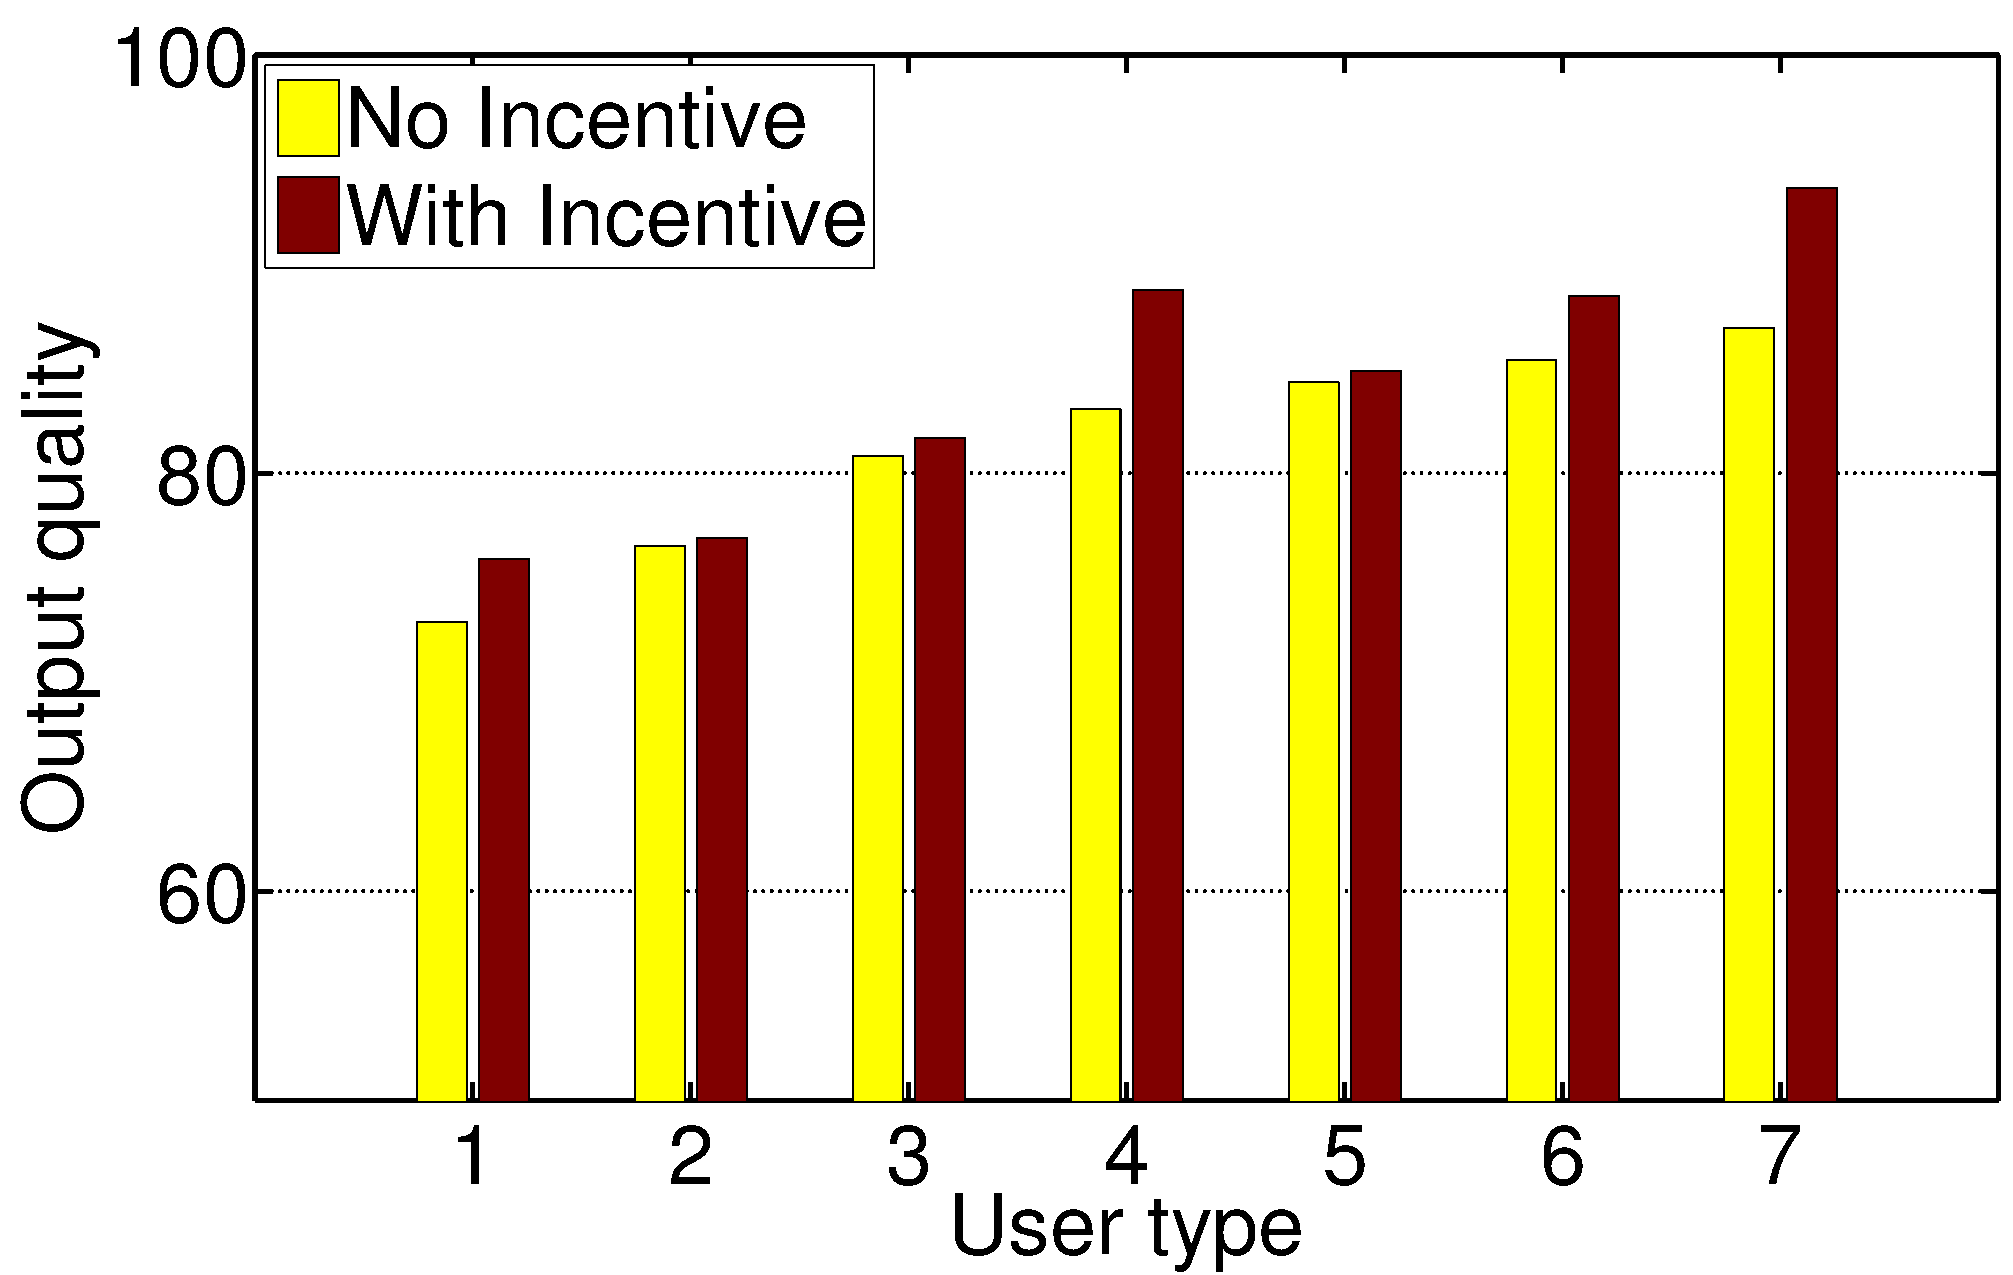
\includegraphics[width=\linewidth]{fig1}
	\caption{1907 Franklin Model D roadster. Photograph by Harris \&
		Ewing, Inc. [Public domain], via Wikimedia
		Commons. (\url{https://goo.gl/VLCRBB}).}
\end{figure}



Your figures should contain a caption which describes the figure to
the reader. Figure captions go below the figure. Your figures should
{\bfseries also} include a description suitable for screen readers, to
assist the visually-challenged to better understand your work.

Figure captions are placed {\itshape below} the figure.

\lipsum[1-2]

\pagestyle{empty}%
\begin{landscape}
	
	\begin{figure}[h]
		\centering
		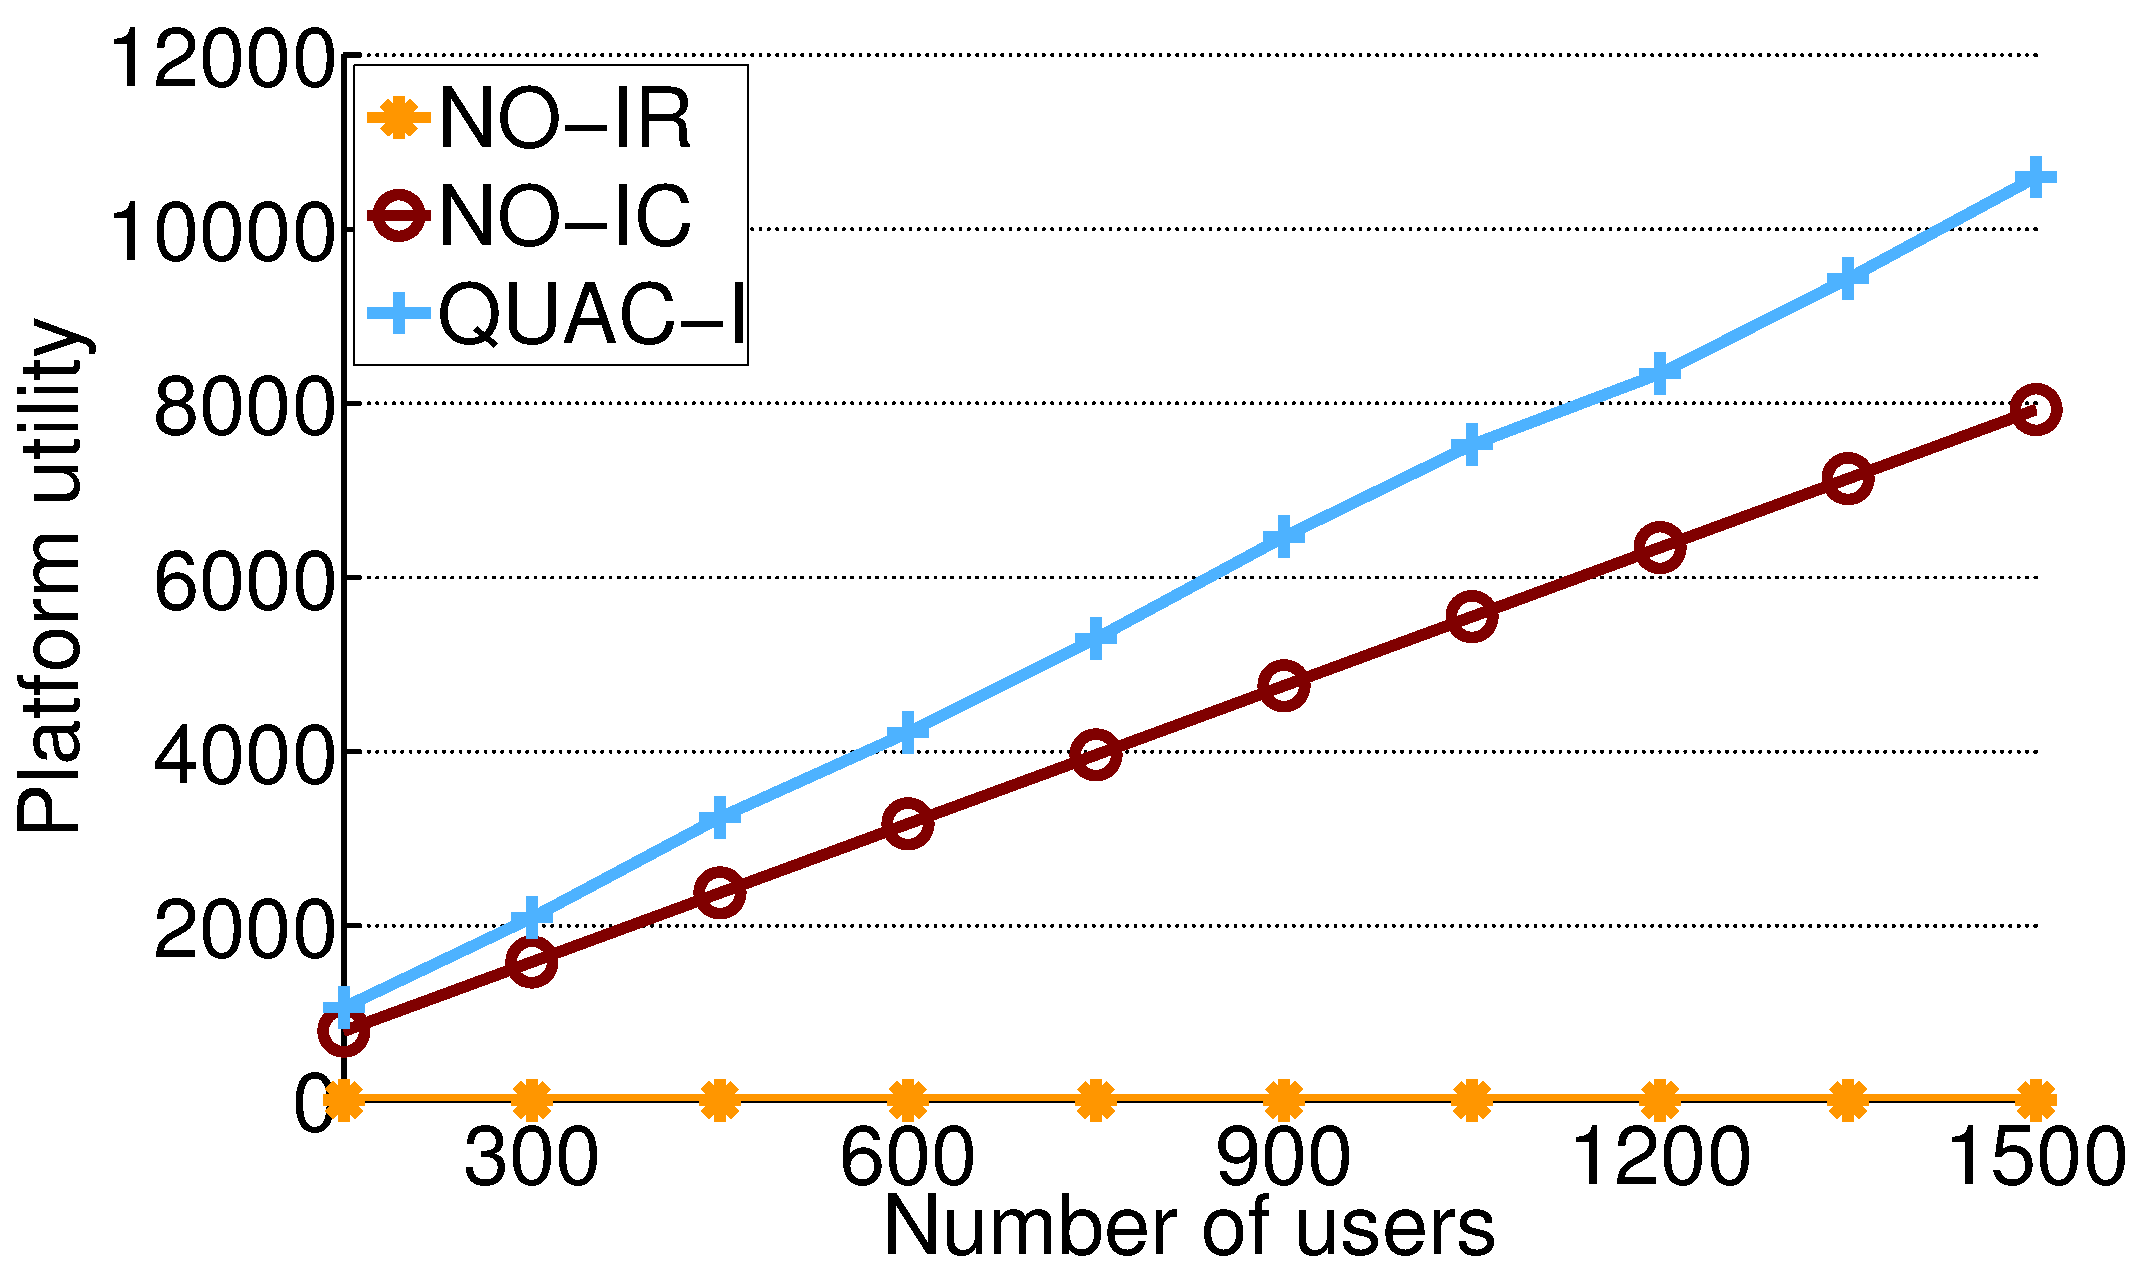
\includegraphics[width=\linewidth]{fig2}
		\caption{1907 Franklin Model D roadster. Photograph by Harris \&
			Ewing, Inc. [Public domain], via Wikimedia
			Commons. (\url{https://goo.gl/VLCRBB}).}
	\end{figure}
\end{landscape}
\pagestyle{plain}%
%========================================
%                            Section                             
%======================================== 
\section{Tables}

The ``\verb|minesthesis|'' document class includes the ``\verb|booktabs|''
package --- \url{https://ctan.org/pkg/booktabs} --- for preparing
high-quality tables.

Table captions are placed {\itshape above} the table.

Because tables cannot be split across pages, the best placement for
them is typically the top of the page nearest their initial cite.  To
ensure this proper ``floating'' placement of tables, use the
environment \textbf{table} to enclose the table's contents and the
table caption.  The contents of the table itself must go in the
\textbf{tabular} environment, to be aligned properly in rows and
columns, with the desired horizontal and vertical rules.  Again,
detailed instructions on \textbf{tabular} material are found in the
\textit{\LaTeX\ User's Guide}.

Immediately following this sentence is the point at which
Table~\ref{tab:freq} is included in the input file; compare the
placement of the table here with the table in the printed output of
this document.

\begin{table}
	\caption{Frequency of Special Characters}
	\label{tab:freq}
	\centering
	\begin{tabular}{ccl}
		\toprule
		Non-English or Math&Frequency&Comments\\
		\midrule
		\O & 1 in 1,000& For Swedish names\\
		$\pi$ & 1 in 5& Common in math\\
		\$ & 4 in 5 & Used in business\\
		$\Psi^2_1$ & 1 in 40,000& Unexplained usage\\
		\bottomrule
	\end{tabular}
\end{table}

To set a wider table, which takes up the whole width of the page's
live area, use the environment \textbf{table*} to enclose the table's
contents and the table caption.  As with a single-column table, this
wide table will ``float'' to a location deemed more
desirable. Immediately following this sentence is the point at which
Table~\ref{tab:commands} is included in the input file; again, it is
instructive to compare the placement of the table here with the table
in the printed output of this document.

\begin{table*}
	\caption{Some Typical Commands}
	\label{tab:commands}
	\centering
	\begin{tabular}{ccl}
		\toprule
		Command &A Number & Comments\\
		\midrule
		\texttt{{\char'134}author} & 100& Author \\
		\texttt{{\char'134}table}& 300 & For tables\\
		\texttt{{\char'134}table*}& 400& For wider tables\\
		\bottomrule
	\end{tabular}
\end{table*}

%========================================
%                            Section                             
%======================================== 
\section{Last section}
\lipsum[6-7]